\documentclass[conference]{IEEEtran}
\IEEEoverridecommandlockouts
% The preceding line is only needed to identify funding in the first footnote. If that is unneeded, please comment it out.
\usepackage{cite}
\usepackage{amsmath,amssymb,amsfonts}
\usepackage{algorithmic}
\usepackage{graphicx}
\usepackage{textcomp}
\usepackage{xcolor}
\usepackage[spanish]{babel}
\usepackage[utf8]{inputenc}
\usepackage{listings}
\usepackage{color}

% A few listings color definition
\definecolor{dkgreen}{rgb}{0,0.6,0}
\definecolor{gray}{rgb}{0.5,0.5,0.5}
\definecolor{mauve}{rgb}{0.58,0,0.82}

% listings definition
\lstset{frame=tb,
	language=Python,
	aboveskip=3mm,
	belowskip=3mm,
	showstringspaces=false,
	columns=flexible,
	basicstyle={\small\ttfamily},
	numbers=none,
	numberstyle=\tiny\color{gray},
	keywordstyle=\color{blue},
	commentstyle=\color{dkgreen},
	stringstyle=\color{mauve},
	breaklines=true,
	breakatwhitespace=true,
	tabsize=3
}

\def\BibTeX{{\rm B\kern-.05em{\sc i\kern-.025em b}\kern-.08em
    T\kern-.1667em\lower.7ex\hbox{E}\kern-.125emX}}

\begin{document}

\title{HMusket: corrector de secuencias mediante el espectro k-mer basado en Hadoop}

\author{\IEEEauthorblockN{1\textsuperscript{st} Luis Lorenzo Mosquera}
\IEEEauthorblockA{\textit{Dpto. de ingeniería de computadores} \\
\textit{GAC (Grupo de Arquitectura de Computadores)}\\
A Coru\~na, Spain \\
luis.lorenzom@udc.es}
\and
\IEEEauthorblockN{2\textsuperscript{nd} Roberto Rey Exposito}
\IEEEauthorblockA{\textit{Dpto. de ingeniería de computadores} \\
\textit{GAC (Grupo de Arquitectura de Computadores)}\\
A Coru\~na, Spain \\
rreye@udc.es}
\and
\IEEEauthorblockN{3\textsuperscript{rd} Jorge González Domínguez}
\IEEEauthorblockA{\textit{Dpto. de ingeniería de computadores} \\
\textit{GAC (Grupo de Arquitectura de Computadores)}\\
A Coru\~na, Spain \\
jgonzaled@udc.es}
}

\maketitle

\begin{abstract}
This document is a model and instructions for \LaTeX.
This and the IEEEtran.cls file define the components of your paper [title, text, heads, etc.]. *CRITICAL: Do Not Use Symbols, Special Characters, Footnotes, 
or Math in Paper Title or Abstract.
\end{abstract}

\begin{IEEEkeywords}
Big Data, Hadoop, Map-Reduce, k-mer, sequence corrector
\end{IEEEkeywords}

\section{Introducción}
Debido a la aparición de la tecnologías conocidas como \textit{Next Generation Sequence} (NGS) se han obtenido grandes volúmenes de datos genéticos procedentes de diversos seres vivos (humanos, animales, plantas, etc). Estos vastos conjuntos de datos se utilizan principalmente para el estudio de los seres vivos secuenciados. 
No obstante con el abaratamiento de estas tecnologías acercan a los científicos hacia nuevos objetivos y metas donde tienen cabida todos estos datos.
\\

Además del ya citado estudio de los seres vivos, otros grandes objetivos o campos de estudios en el área de las ciencias de la vida (biología, medicina, etc.) es la predicción de enfermedades, de carácter o predisposición genética, en un estadío temprano para evitar futuras complicaciones en el paciente. \\
La evasión del fraude en productos alimenticios, tanto para detectar la procedencia u origen del producto en cuestión es otro de las grandes áreas de estudio principalmente por el tema comercial.\\
Por último, la interacción de la información contenida en los datos obtenidos durante la fase de secuenciación junto con una base de conocimiento tanto de las áreas de la farmacología y patología da como resultado la farmacogenética, pudiendo predecir qué fármaco es más efectivo, ideal o quizás poder diseñar un fármaco para un individuo.
\\

No obstante para llegar a tales fines y obtener unos resultados adecuados son necesarios una serie de pasos previos. Además de obtener una muestra de ADN y secuenciarla es necesario corregir ese conglomerado de datos, ya que durante la fase de amplificación/síntesis de nuevas copias por PCR es posible que se incorporen errores debido a fallos de ADN polimerasa.\\ Afortunadamente esta clase de fallos siguen un proceso estocástico y pueden ser corregidas por medio de diversos algoritmos.
\\

Debido a la problemática indicando en el párrafo superior junto con la gran demanda de datos genéticos que se están sucediendo las soluciones tradicionales para corregir los errores generados durante la fase de amplificación producen un cuello de botella a la hora de emplear esos datos ya que la mayoría de estas soluciones son secuenciales o de memoria compartida no logran reducir considerablemente los tiempos de pre-procesado de los datos.
\\

En el propósito de este trabajo es de proveer a los científicos una herramienta de memoria distribuida que pueda reducir el tiempo de corrección de las secuencias, además de esto, en este trabajo se realiza una análisis de las herramientas que hay disponibles en el mercado (tanto de memoria compartida como distribuida) una introducción y explicación de las tecnologías utilizadas a lo largo del proyecto, para posteriormente detallar el diseño y la implementación del software aquí expuesto, y finalizando con una serie de resultados donde se muestran una comparativa de tiempos y unas conclusiones

\section{Trabajos relacionados}

A lo largo de esta sección se presentarán las diferentes soluciones que hay actualmente en el mercado para la tarea de corregir las secuencias además de indicar tanto sus bondades y sus defectos.

\subsection{Memoria compartida}

Dentro del grupo de soluciones de memoria compartida cabe destacar las soluciones basada en GPU como son CUDE-EC y DecGPU las cuales utilizan un algoritmo basado en efectuar lecturas cortas del genoma lo que no provee una solución completa de errores ni una alta precisión en los resultados, no obstante al estar desarrolladas para GPUs presentan una índice de escalabilidad alto.\\

Otra solución que utiliza un algoritmo basado en lecturas cortas del genoma usando en este caso CPU en lugar de GPU es SOAP corrector. Posteriores versiones del algoritmo utilizan para determinadas operaciones un método basado en el grafo De Brujin, lo cual reduce drásticamente el uso de memoria en casos casos donde la longitud del genoma pueda presentar problemas.\\

Siguiendo con las soluciones que utilizan o están basadas en modelos de grafos, se encuentra Reptile, este software hace uso de un grafo Hamming para resolver las posibles ambigüedades que se encuentren en el genoma o región genómica a corregir, muy útil en casos que presenten errores de translocación.\\

Sin ser un software basado en un modelo de grafos, SGA consigue optimizar el uso de la memoria utilizando la tranformada de Burrows-Wheeler y el FM-Index para representar el espectro k-mer de la región genómica.\\

Además de los métodos de lecturas cortas y métodos basados en grafos hay alternativas basadas en modelos probabilísticos como por ejemplo: Quake, este corrector utiliza la probabilidad acumulada de los k-mer que conforman el genoma para poder clasificar si se trata de un error o no.\\

También existen soluciones que combinan dos posibles como por ejemplo: Hammer que se compone de una solución basada en un grafo Hamming y un modelo probabilístico de la probabilidad acumulada de los k-mer, al igual que hace Quake.\\

Por último indicar correctores que hacen uso de arrays de sufijos como son HiTEC, el cual instancia el genoma con distintos k-mers para posteriormente crear esos arrays y analizar los errores, o SHREC que utiliza un método parecido por HiTEC pero para la detección de indels y sustituciones.\\

%%%%%%%%%%%%%%%%%%%%%%%%%%%%%%%%%%%%%%%%%%%%%
%%%%%%%%%%%% TODO %%%%%%%%%%%%%%%%%%%%%%%%%%%
%%%%%%%%%%%%%%%%%%%%%%%%%%%%%%%%%%%%%%%%%%%%%
\subsection{Memoria distribuida}

The IEEEtran class file is used to format your paper and style the text. All margins, 
column widths, line spaces, and text fonts are prescribed; please do not 
alter them. You may note peculiarities. For example, the head margin
measures proportionately more than is customary. This measurement 
and others are deliberate, using specifications that anticipate your paper 
as one part of the entire proceedings, and not as an independent document. 
Please do not revise any of the current designations.\\	

Quake\\

Cloud-CRS

\section{Conocimiento previo}

A lo largo de esta sección se expondrán y detallarán brevemente las diversas tecnologías utilizadas en este proyecto.

\subsection{Hadoop}
Framework, de código abierto, desarrollado en Java el cual esta orientado a la ejecución de aplicaciones distribuidas en un entorno clúster y al procesamiento de forma eficiente de grandes conjuntos de datos. Proveyendo de un ecosistema que permite a otras aplicaciones comunicarse entre si, hacer uso del mismo sistema de recursos (YARN) o de compartir el sistema de ficheros distribuido (HDFS).

\subsection{Map-Reduce}
Modelo de programación que surge ante la necesidad de procesar cantidades ingentes de datos. Este paradigma consta de dos operaciones.\\

La operación Map convierte un par (clave, valor) en otro conjunto intermedio de datos en el mismo formato de tupla. Este formato de tupla hace mucho mas eficiente el procesado de los datos y una futura reconstrucción de los mismos.\\

\begin{lstlisting}
# Se inicializa un dataset con unos valores
dataset = [1, 2, 3, 4, 5]
# Se realiza la operacion de elevar al 
# cuadrado, mediante una funcion lambda
# y el resultado se almacena como una lista
dataset = list(map(lambda x: x**2, dataset))
# dataset = [1, 4, 9, 16, 25]
\end{lstlisting}

La operación Reduce utiliza los conjuntos de datos intermedios generados por las operaciones Map para agruparlos y mostrar un resultado final.

\begin{lstlisting}
# Se inicializa un dataset con unos valores
dataset = [1, 2, 3, 4, 5]
# Al igual que en el ejemplo anterior se utiliza una
# funcion lambda, en este caso la multiplicacion de dos numeros
value = reduce((lambda x, y: x * y), dataset)
# value = 120
\end{lstlisting}

\subsection{HDFS}
Sistema de ficheros distribuido que permite ejecutar las aplicaciones del ecosistema Hadoop con una alta tolerancia a fallos, además de facilitar el acceso de los datos a todo el conjunto de computadores que componen el clúster.

\subsection{HSP}
Hadoop Sequence Parser (HSP) es una librería desarrollada en Java para el parseo de datasets en formato Fasta o Fastq almacenados en Hadoop Distributed File System (HDFS).

\subsection{JNI}
Framework que permite que un determinado código Java ejecutado sobre la JVM ejecute y reciba llamadas desde código nativo, es decir, programas y/o librerías desarrolladas en C, C++ o Assembler.

\subsection{Musket}
Software que permite la corrección de conjuntos de datos secuencias genómicas en base al espectro k-mer de las mismas, este programa esta acelerado mediante la API de OpenMP pudiendo paralelizar parte de su pipeline de corrección genómica entre los distintos cores de la máquina donde se esta ejecutando.\\
Para realizar dicha aceleración los desarrolladores del software decidieron abordar este problema utilizando un patrón maestro esclavo, por el cual sigue un proporción de x maestros frente a y esclavos para evitar cualquier tipo de cuello de botella. Además de lo ya citado anteriormente este corrector ofrece, gracias al uso del análisis del espectro k-mer una gran cobertura de todo el código genético procesado.

\section{Diseño e implementación}

Para el desarrollo del presente trabajo se tuvieron que completar pequeños hitos que componen la totalidad del dicho proyecto, a continuación se detallan con total exactitud en que consistieron tales hitos, es decir, comentar el problema que le dio origen y que solución/estrategias se utilizaron para alcanzar la solución.\\

En lineas generales lo se busca en este proyecto es distribuir entre varios nodos un determinado dataset ya sea fasta o fastq en modo single-end o pair-end y ejecutar varias instancias del software musket para finalmente hacer un merge de todas las salidas.\\

No obstante antes de entrar en detalle, se dará una visión general de como son las aplicaciones map/reduce.

\subsection{Estructura general}
Las aplicaciones Map/Reduce, por lo general, consiste en: un driver donde se configura la aplicación (ficheros de entrada, salida, formatos con los que va a trabajar, etc), se crea un job, al cual se le indican los mappers y los reducers con los que va a trabajar. Junto con el driver se tienen que implementar las clases Map y Reduce que se le indican en el driver siguiendo un ``ciclo de vida'' en ambos casos:

\begin{itemize}
	\item Set up: operación que se realiza al inicio de la etapa map o reduce
	\item Map o Reduce: operación/función que se realizada por cada par (clave, valor) del conjunto de datos a manejar.
	\item Clean up: operación que se realiza al inicio de la etapa map o reduce.
\end{itemize}

Una vez detallado la estructura de una aplicación map/reduce se puede detallar como funciona y como esta organizado HMusket.

\subsection{Desarrollo de la aplicación Map/Reduce}
HMusket sigue la estructura indicada en el aparatado anterior, en el driver se recogen los parámetros de entrada y se invoca el método parse de la clase CLIParse para evaluar la obligatoriedad de los parámetros de entrada, configurar el driver utilizando los parámetros de entrada y generar un string que conforme los argumentos que recibirá musket para corregir las secuencias del dataset.\\
Una vez configurado el driver establece los ficheros de entrada y salida de los mappers, en este caso hace uno de las clases InputFormat de la librería HSP, de esta manera cada mapper recibe un parte proporcional del dataset, en el caso de los fastq, se recibe por cada secuencia el id, la cadena de las bases nitrogenadas y los indicadores de calidad, sin tener que modificar el formato del fichero de entrada, tan solo subiéndolo previamente a HDFS.\\
Los distintos mappers que se manejan en esta aplicación durante la fase de setup instancian un printWriter para posteriormente en la etapa map poder volcar toda la información a disco duro local del nodo de computo. Finalmente en la etapa cleanup se cierra el buffer de escritura del printWriter y se llama al método callMusket de la clase MusketCaller, que previamente a cargado en memoria la librería estática donde esta la funcionalidad de musket, el string que conforma los argumentos de musket generado en el método parse de la clase CLIParse. Finalmente elimina los archivos locales que se utilizaron para la ejecución de musket y se suben a HDFS para que simplemente se tenga que hacer un merge de los mismos.

%\begin{figure}[htbp]
%	\centerline{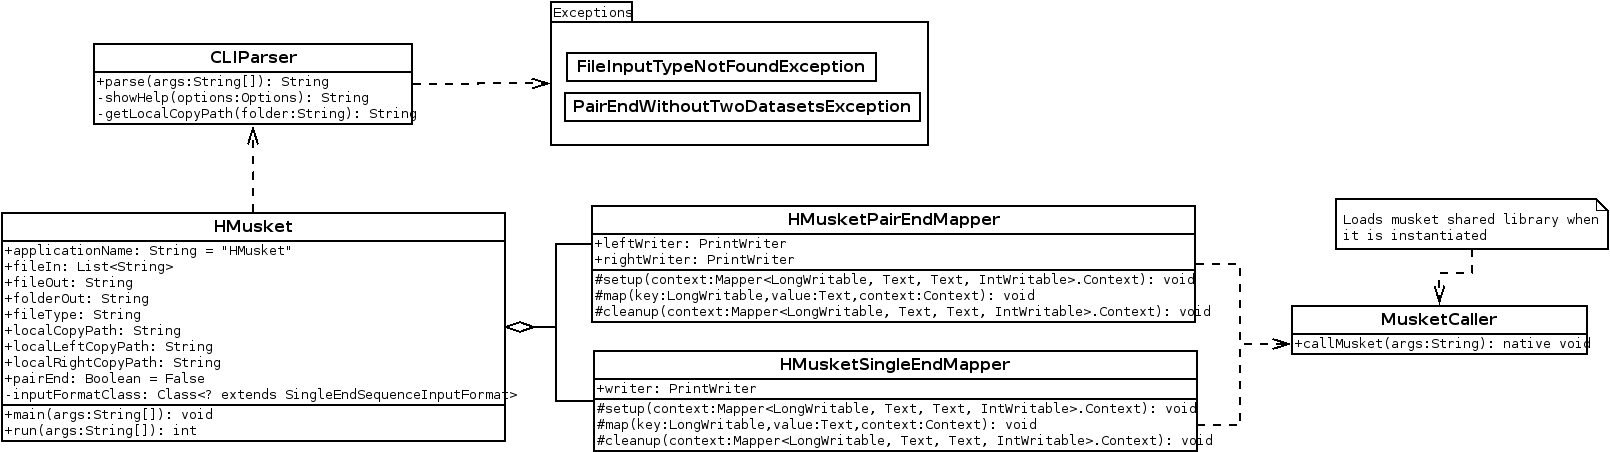
\includegraphics[width=20cm,height=5cm]{figures/hmusket.png}}
%	\caption{Diagrama de clases de HMusket}
%	\label{fig}
%\end{figure}

\subsection{Creación e integración de la librería}
Para poder realizar la llamada a código nativo lo primero de todo es convertir el software musket en una shared library para posteriormente instalarla en el clúster hadoop y que  de esta manera cualquier programa del ecosistema hadoop puede hacer uso de la misma.\\
Para llevar a cabo esta tarea lo primero de todo es crear una clase en el proyecto Java, en este caso fue en la clase MusketCaller, donde se especifique que durante la fase de instanciación cargue la librería nativa, en el caso del presente proyecto la librería ``musket'', además de esta indicación se tiene que crear un método con la etiqueta ``native'', que al igual que en los métodos abstractos tan solo se debe especificar la firma.\\
A continuación utilizando el comando ``javac'' se compila dicha generando un fichero .class, este fichero es requerido para generar el header file (.h), por medio del comando ``javah'' para posteriormente darle una implementación en un programa C.\\
Finalmente se tiene que desarrollar un programa en C o C++ donde se incluya el header file generado en el paso anterior y la librería de JNI, darle implementación a la función indicada en el header file y finalmente realizar la llamada de musket.\\
Para poder realizar una llamada a musket como si fuera una librería en vez de un binario se tiene que modificar el makefile del software en cuestión para añadir los parámetros ``-fPIC'' y ``-shared'' para la creación de esta librería. Una vez creada la librería se tiene que añadir al directorio \$HADOOP\_HOME/lib/native y por último declarar la función main dentro del programa C que implemente el header generado.

\section{Evaluación experimental}
A lo largo de esta sección se detallará el entorno, tanto software como hardware, donde se realización de las pruebas, los distintos experimentos llevados a cabo y una serie de comentarios acerca de los resultados obtenidos.

\subsection{Entorno de pruebas}
Para la realización de las diversas pruebas expuestas en los siguientes párrafos se utilizó el clúster Plutón del departamento de ingeniería de computadores el cual consta con 18 nodos de cómputo de la siguientes características: 

\begin{itemize}
	\item \textbf{CPU Model}: 2 × Intel Xeon E5-2660 Sandy Bridge-EP
	\item \textbf{CPU Speed/Turbo}: 2.20 GHz/3 GHz
	\item \textbf{Cores por CPU}: 8
	\item \textbf{Threads por core}: 2
	\item \textbf{Cores/Threads por nodo}: 16/32
	\item \textbf{Cache L1/L2/L3}: 32 KB/256 KB/20 MB
	\item \textbf{Memoria RAM}: 64 GB DDR3 1600 Mhz
	\item \textbf{Discos}: 1 × HDD 1 TB SATA3 7.2K rpm y 1 × SSD 480 GB SATA3 (de los nodos 8 a 15)
	\item \textbf{Redes}: InfiniBand FDR y Gigabit Ethernet
\end{itemize}

En resumen, el clúster cuenta con 1 nodo de login y 18 nodos de cómputo con un total de 288 cores físicos (576 threads), 1.152 TB de memoria.\\

El sistema operativo que se ejecuta en esta máquina es Rocks 6.1 una distribución para entornos cluster basada en CentOS 6.

%%%%%%%%%%%%%%%%%%%%%%%%%%%%%%%%%%%%%%%%%%%%%
%%%%%%%%%%%% TODO %%%%%%%%%%%%%%%%%%%%%%%%%%%
%%%%%%%%%%%%%%%%%%%%%%%%%%%%%%%%%%%%%%%%%%%%%
\subsection{Análisis Musket}

\subsection{Análisis HMusket}

\section{Conclusiones y trabajo futuro}

\section*{Referencias bibliográficas}

Please number citations consecutively within brackets \cite{b1}. The 
sentence punctuation follows the bracket \cite{b2}. Refer simply to the reference 
number, as in \cite{b3}---do not use ``Ref. \cite{b3}'' or ``reference \cite{b3}'' except at 
the beginning of a sentence: ``Reference \cite{b3} was the first $\ldots$''

Number footnotes separately in superscripts. Place the actual footnote at 
the bottom of the column in which it was cited. Do not put footnotes in the 
abstract or reference list. Use letters for table footnotes.

Unless there are six authors or more give all authors' names; do not use 
``et al.''. Papers that have not been published, even if they have been 
submitted for publication, should be cited as ``unpublished'' \cite{b4}. Papers 
that have been accepted for publication should be cited as ``in press'' \cite{b5}. 
Capitalize only the first word in a paper title, except for proper nouns and 
element symbols.

For papers published in translation journals, please give the English 
citation first, followed by the original foreign-language citation \cite{b6}.

\begin{thebibliography}{00}
\bibitem{b1} G. Eason, B. Noble, and I. N. Sneddon, ``On certain integrals of Lipschitz-Hankel type involving products of Bessel functions,'' Phil. Trans. Roy. Soc. London, vol. A247, pp. 529--551, April 1955.
\bibitem{b2} J. Clerk Maxwell, A Treatise on Electricity and Magnetism, 3rd ed., vol. 2. Oxford: Clarendon, 1892, pp.68--73.
\bibitem{b3} I. S. Jacobs and C. P. Bean, ``Fine particles, thin films and exchange anisotropy,'' in Magnetism, vol. III, G. T. Rado and H. Suhl, Eds. New York: Academic, 1963, pp. 271--350.
\bibitem{b4} K. Elissa, ``Title of paper if known,'' unpublished.
\bibitem{b5} R. Nicole, ``Title of paper with only first word capitalized,'' J. Name Stand. Abbrev., in press.
\bibitem{b6} Y. Yorozu, M. Hirano, K. Oka, and Y. Tagawa, ``Electron spectroscopy studies on magneto-optical media and plastic substrate interface,'' IEEE Transl. J. Magn. Japan, vol. 2, pp. 740--741, August 1987 [Digests 9th Annual Conf. Magnetics Japan, p. 301, 1982].
\bibitem{b7} M. Young, The Technical Writer's Handbook. Mill Valley, CA: University Science, 1989.
\end{thebibliography}

\end{document}
